\documentclass{article}

\usepackage{microtype}
\usepackage{graphicx}
\usepackage{booktabs}
\usepackage{amsmath}
\usepackage{amssymb}
\usepackage{xcolor}
\usepackage{multirow}

\usepackage{hyperref}

\newcommand{\theHalgorithm}{\arabic{algorithm}}

\usepackage[preprint,nohyperref]{icml2026}

\usepackage{mathtools}
\usepackage{amsthm}

\icmltitlerunning{Representational Commitment: Hidden States Predict Agent Consistency}

\begin{document}

\twocolumn[
\icmltitle{Representational Commitment: \\ When Hidden States Predict Behavioral Consistency in LLM Agents}

\icmlsetsymbol{equal}{*}

\begin{icmlauthorlist}
\icmlauthor{Aman Mehta}{sf}
\end{icmlauthorlist}

\icmlaffiliation{sf}{Snowflake Inc.}

\icmlcorrespondingauthor{Aman Mehta}{aman.mehta@snowflake.com}

\icmlkeywords{LLM agents, behavioral consistency, hidden states, interpretability, representational analysis}

\vskip 0.3in
]

\printAffiliationsAndNotice{}

\begin{abstract}
LLM-based agents exhibit behavioral inconsistency: the same agent given the same task produces different reasoning trajectories across runs. We investigate whether this inconsistency has a signature in internal representations. Using Llama-3.1-70B on a ReAct question-answering task (100 questions, 10 runs each), we find that \emph{activation similarity}---pairwise cosine similarity of hidden states across runs---predicts behavioral consistency ($r = -0.35$, permutation $p < 0.001$). Counterintuitively, higher similarity predicts \emph{less} consistency: undifferentiated hidden states indicate the model has not committed to a strategy, and future behavior diverges. This signal emerges at step~4, spans layers 32--80, strengthens after controlling for difficulty (partial $r = -0.45$, $p < 10^{-5}$), and is not explained by simple baselines. It predicts between-run consistency but not per-run correctness (AUC~$\approx 0.6$). To our knowledge, this is the first work connecting agent behavioral consistency to hidden-state geometry.
\end{abstract}

\section{Introduction}

LLM-based agents---systems combining language models with tool use and multi-step reasoning \citep{react, cot}---face a critical reliability concern: \emph{behavioral inconsistency}, where the same agent given the same input produces different outputs across runs \citep{mehta2026agents, mehta2026consistency}. While prior work characterized this inconsistency behaviorally, a fundamental question remains: \emph{does consistency have a signature in the model's internal representations?}

We answer affirmatively. Extracting hidden states from Llama-3.1-70B \citep{llama3} during ReAct \citep{react} question-answering on HotpotQA \citep{hotpotqa}, we find that cross-run \emph{activation similarity} at a critical reasoning step predicts behavioral consistency. We call this \textbf{representational commitment}: when hidden states differentiate in response to observations, downstream behavior is consistent; when they remain undifferentiated, behavior diverges. Our contributions:
\begin{enumerate}
\item Activation similarity at step~4 predicts consistency ($r = -0.35$, permutation $p < 0.001$, $n{=}100$), \emph{strengthening} after difficulty controls (partial $r = -0.45$, $p < 10^{-5}$).
\item The signal is temporally and spatially specific: absent at steps 1--2, peaking at step~4, spanning layers 32--80.
\item The signal predicts \emph{between-run consistency} but not \emph{per-run correctness} (AUC~$\approx 0.6$).
\end{enumerate}

\section{Related Work}

\textbf{Behavioral consistency.} \citet{mehta2026agents} introduced behavioral consistency as an agent reliability metric; \citet{mehta2026consistency} showed it predicts accuracy. Self-consistency \citep{wang2023selfconsistency} uses output-level variance for majority voting but does not examine internal representations. \citet{elazar2021consistency} studied token-level consistency in non-agentic settings.

\textbf{Probing hidden states.} LLM hidden states encode truth \citep{burns2023discovering, marks2024geometry}, support inference-time intervention \citep{li2024inference}, distinguish truthful from deceptive outputs \citep{azaria2023internal}, and encode model confidence \citep{kadavath2022language, stickland2024reasoning}. We extend probing to \emph{behavioral consistency in agentic settings}.

\textbf{Representation engineering.} \citet{zou2023repe} introduced representation engineering; \citet{turner2023steering} demonstrated activation steering; \citet{templeton2024scaling} extracted interpretable features at scale. We identify \emph{where} consistency information lives, informing future interventions.


\section{Method}

\textbf{Setup.} We use Llama-3.1-70B \citep{llama3} in a ReAct \citep{react} agent on HotpotQA \citep{hotpotqa}. The agent iterates Thought $\rightarrow$ Action $\rightarrow$ Observation using Search, Retrieve, and Finish tools. We select 100 questions (50 easy, 50 hard), run each 10 times ($T{=}0.6$, 988 total runs), and extract hidden states $\mathbf{h}_{\ell}^{(s)} \in \mathbb{R}^{8192}$ from the last token at layer $\ell \in \{0, 8, \ldots, 80\}$ and step $s \in \{1, \ldots, 5\}$.

\textbf{Metrics.} \emph{Behavioral consistency} (CV): coefficient of variation of step count across 10 runs. \emph{Activation similarity}: mean pairwise cosine similarity of hidden states across runs at a given step and layer:
$\text{Sim}_q^{(s,\ell)} = \binom{n}{2}^{-1} \sum_{i < j} \cos(\mathbf{h}_{\ell,i}^{(s)}, \mathbf{h}_{\ell,j}^{(s)})$.
We examine the Pearson correlation between $\text{Sim}_q^{(s,\ell)}$ and $\text{CV}_q$ across questions.


\section{Results}

\subsection{Core Finding: Activation Similarity Predicts Consistency}

Figure~\ref{fig:heatmap} shows the correlation between activation similarity and behavioral CV across all step--layer combinations. A strong negative correlation emerges at step~4 across layers 32--80, peaking at layer~40 ($r = -0.35$, $p = 0.0006$). The sign is counterintuitive: higher similarity predicts \emph{higher} CV (more inconsistent behavior). A 10{,}000-permutation test confirms all seven layers from 32 to 80 are significant ($p < 0.002$; Table~\ref{tab:permutation}).

\begin{figure}[t]
\centering
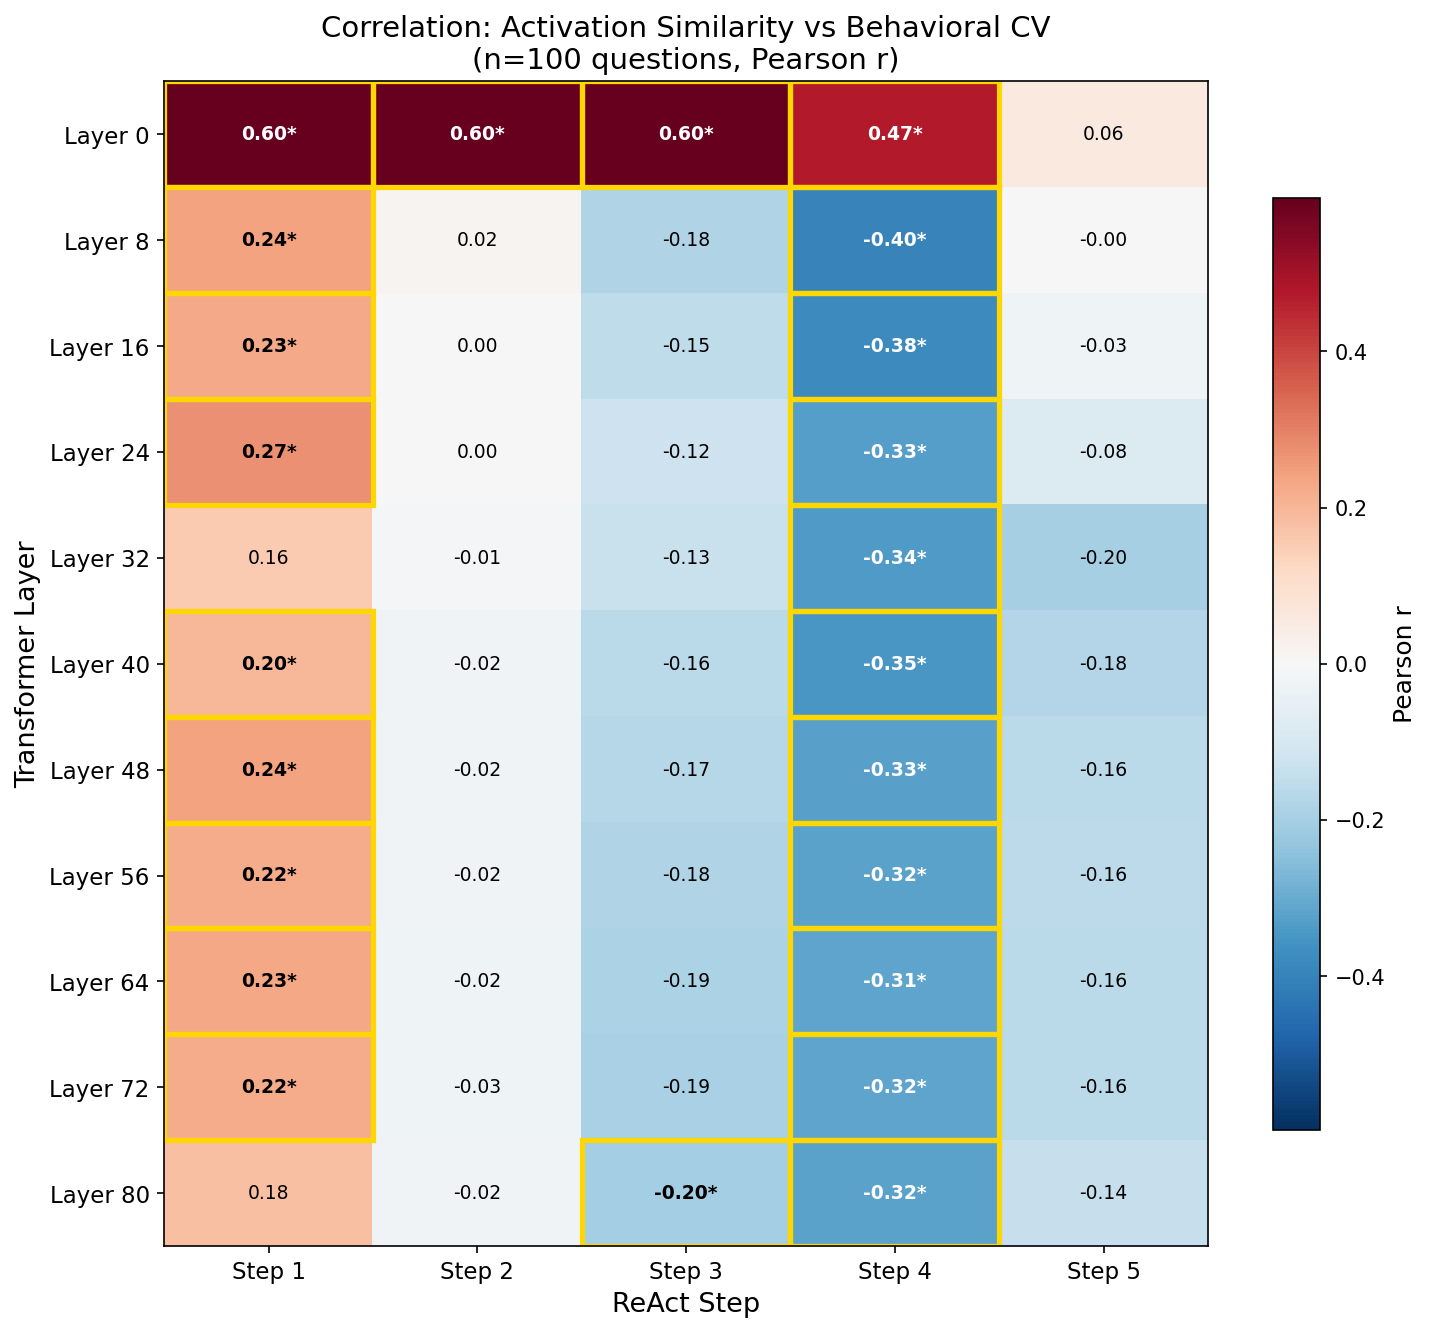
\includegraphics[width=\columnwidth]{figures/step_layer_heatmap_100q.png}
\caption{Pearson $r$ between activation similarity and behavioral CV ($n = 99$). Gold borders: $p < 0.05$. Signal emerges at step~4 across layers 32--80.}
\label{fig:heatmap}
\end{figure}

\begin{table}[t]
\caption{Permutation test at step~4 ($n = 94$, 10{,}000 permutations).}
\label{tab:permutation}
\centering
\small
\begin{tabular}{lccc}
\toprule
Layer & $r$ & Param.\ $p$ & Perm.\ $p$ \\
\midrule
32 & $-0.340$ & $0.0008$ & $0.0007$ \\
\textbf{40} & $\mathbf{-0.347}$ & $\mathbf{0.0006}$ & $\mathbf{0.0003}$ \\
48 & $-0.326$ & $0.0013$ & $0.0012$ \\
56 & $-0.320$ & $0.0017$ & $0.0011$ \\
64 & $-0.313$ & $0.0021$ & $0.0014$ \\
72 & $-0.316$ & $0.0019$ & $0.0019$ \\
80 & $-0.319$ & $0.0017$ & $0.0019$ \\
\bottomrule
\end{tabular}
\end{table}

\textbf{Interpretation.} When runs update their hidden states differently in response to observations---producing low cross-run similarity---they have ``committed'' to distinct strategies and proceed consistently. When hidden states remain similar despite different observations, runs are ``uncommitted'' and downstream behavior diverges.


\subsection{Temporal Profile}

Figure~\ref{fig:step_progression} shows the correlation at layer~40 across steps. The signal is absent at steps 1--2, strengthens at step~3, peaks at step~4 ($r = -0.35$), and weakens at step~5. Step~1 shows a weak positive correlation ($r = 0.20$, $p = 0.048$), possibly reflecting question-encoding effects. The signal appears precisely when the model has enough evidence to differentiate strategies.

\begin{figure}[t]
\centering
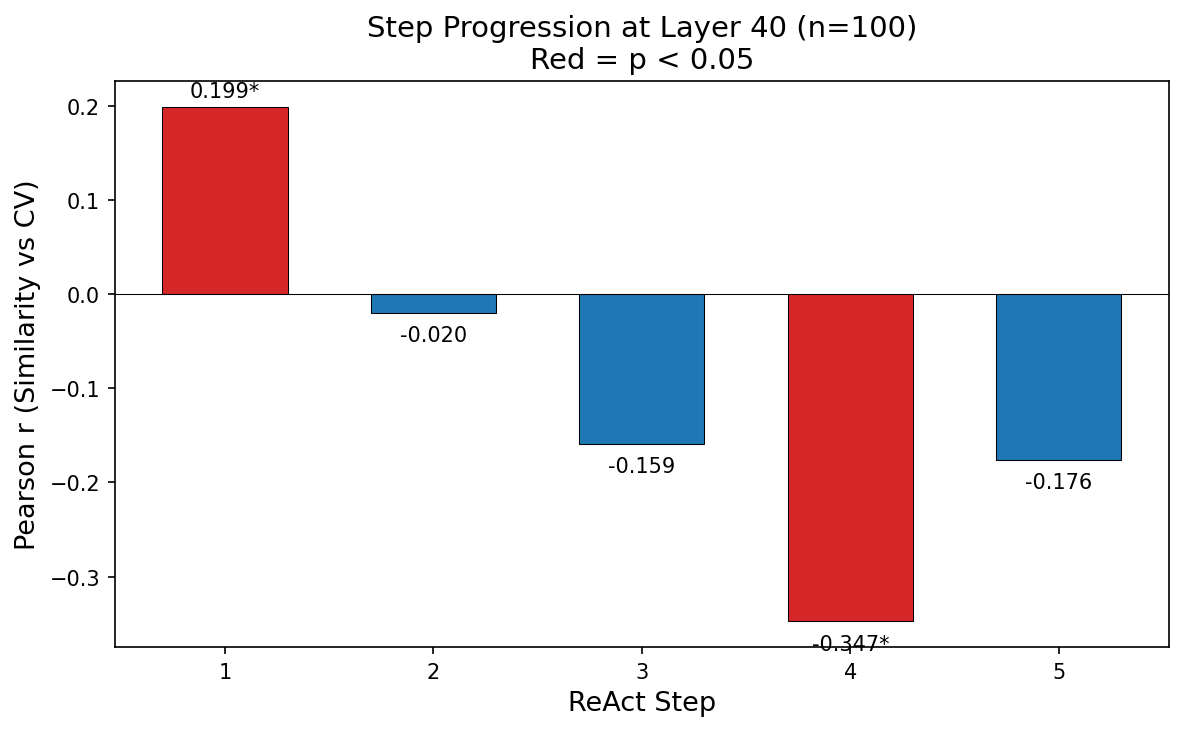
\includegraphics[width=\columnwidth]{figures/step_progression_layer40_100q.png}
\caption{Correlation at layer~40 across steps. The signal peaks at step~4.}
\label{fig:step_progression}
\end{figure}


\subsection{Controlling for Task Difficulty}

Both similarity and CV could reflect task difficulty. Partial correlation controlling for accuracy and difficulty label shows the signal \emph{strengthens}: raw $r = -0.35$ becomes partial $r = -0.45$ ($p < 10^{-5}$; Figure~\ref{fig:partial}). Accuracy acts as a suppressor variable; all layers survive (Table~\ref{tab:partial}).

\begin{figure}[t]
\centering
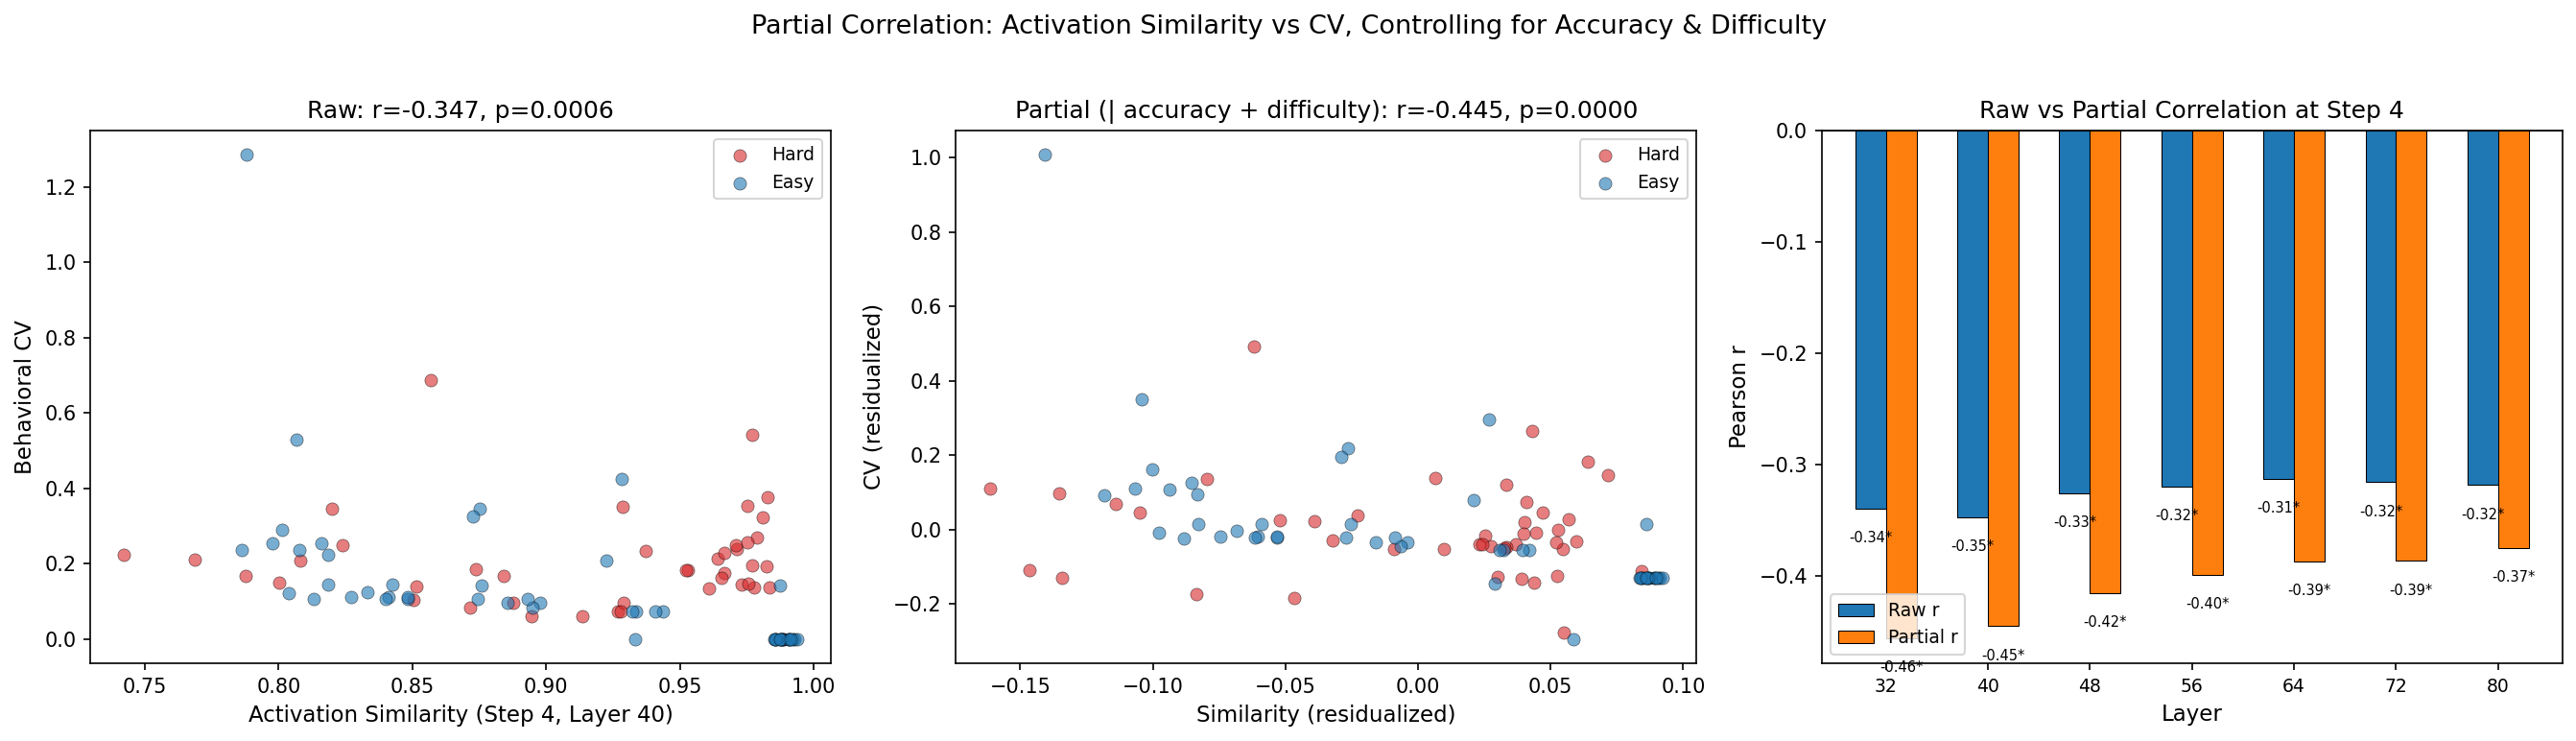
\includegraphics[width=\columnwidth]{figures/partial_correlation_step4.png}
\caption{Partial correlation analysis. \textbf{Left:} Raw scatter colored by difficulty. \textbf{Center:} After residualizing on accuracy and difficulty ($r{:}\;{-}0.35 \to {-}0.45$). \textbf{Right:} Raw vs.\ partial $r$ across layers.}
\label{fig:partial}
\end{figure}

\begin{table}[t]
\caption{Partial correlations at step~4, controlling for accuracy and difficulty.}
\label{tab:partial}
\centering
\small
\begin{tabular}{lcccc}
\toprule
Layer & Raw $r$ & Raw $p$ & Partial $r$ & Partial $p$ \\
\midrule
32 & $-0.340$ & $.0008$ & $-0.456$ & $< .0001$ \\
\textbf{40} & $\mathbf{-0.347}$ & $\mathbf{.0006}$ & $\mathbf{-0.445}$ & $< \mathbf{.0001}$ \\
48 & $-0.326$ & $.0013$ & $-0.416$ & $< .0001$ \\
56 & $-0.320$ & $.0017$ & $-0.399$ & $< .0001$ \\
64 & $-0.313$ & $.0021$ & $-0.387$ & $.0001$ \\
72 & $-0.316$ & $.0019$ & $-0.387$ & $.0001$ \\
80 & $-0.319$ & $.0017$ & $-0.375$ & $.0002$ \\
\bottomrule
\end{tabular}
\end{table}


\subsection{Ruling Out Simple Baselines}

Table~\ref{tab:baselines} compares predictors of CV. Question length ($r = 0.10$, $p = 0.31$) and context size ($r = 0.04$, $p = 0.66$) are not significant. Behavioral features (step count, thought length) show weak correlations but are downstream consequences. Multiple regression (CV $\sim$ similarity + question length + accuracy) yields $R^2 = 0.30$; similarity ($t = -4.73$, $p < 10^{-5}$) and accuracy ($t = -4.41$, $p < 10^{-4}$) are the only significant predictors.

\begin{table}[t]
\caption{Predictors of behavioral CV. $*$: $p < 0.05$.}
\label{tab:baselines}
\centering
\small
\begin{tabular}{lrr}
\toprule
Predictor & $r$ & $p$ \\
\midrule
\textbf{Hidden-state sim.\ (S4, L40)} & $\mathbf{-0.35}$ & $\mathbf{.0006}$ \\
Accuracy (correct rate) & $-0.31$ & $.002$ \\
Mean total thought length & $0.26$ & $.011$ \\
Mean search actions & $0.23$ & $.019$ \\
Mean step count & $0.21$ & $.037$ \\
\midrule
Question word count & $0.10$ & $.31$ \\
N context documents & $0.04$ & $.66$ \\
\bottomrule
\end{tabular}
\end{table}


\subsection{Boundaries}

\textbf{Per-run correctness.} A nearest-centroid classifier achieves AUC~$\approx 0.61 \pm 0.05$ for distinguishing consistently-correct questions---modestly above chance. The signal predicts \emph{consistency}, not \emph{correctness}.

\textbf{Hard vs.\ easy questions.} The signal is driven by easy questions ($r = -0.57$, $p < 10^{-5}$, $n = 50$) rather than hard ($r = -0.02$, $p = 0.88$, $n = 44$). Leave-one-out analysis confirms robustness within the easy subset (all 50 iterations significant, $r \in [-0.67, -0.55]$). Hard questions may lack sufficient variance for the signal to manifest.


\section{Discussion}

\textbf{Why does high similarity predict inconsistency?} When all runs produce similar hidden states despite receiving different observations, the model has not committed to a strategy. These undifferentiated representations are fragile: sampling perturbations have no anchor, and trajectories diverge. When observations produce different hidden states, each run has integrated evidence into a committed representation that guides consistent behavior.

\textbf{Why step~4?} Steps 1--3 involve initial queries with limited information. By step~4, the model has received 3--4 observations and must integrate them. This is the commitment juncture. The signal fading at step~5 reflects trajectories having already diverged.

\textbf{Implications and limitations.} This opens a direction connecting agent reliability to internal representations, with applications in monitoring (flagging uncommitted states), intervention (activation steering), and architecture design. Our study is limited to one model, one task, and one consistency measure. The causal direction is uncertain, and the hard-question null result limits generalizability.

\section{Conclusion}

Behavioral consistency in LLM agents has a measurable internal signature. At step~4 of a ReAct trajectory (layers 32--80), the degree to which hidden states differentiate across runs predicts downstream consistency. This signal survives difficulty controls, is not explained by simple baselines, and predicts consistency but not correctness.

\bibliography{references}
\bibliographystyle{icml2026}

\end{document}
